\documentclass[12pt,a4paper]{article}

\usepackage[croatian]{babel}
\usepackage[utf8]{inputenc}
\usepackage[hyphens]{url}

\usepackage{graphicx}

\usepackage[margin=2cm]{geometry}
\usepackage[colorlinks=true,urlcolor=black]{hyperref}
\pagenumbering{gobble}

\begin{document}
	\title{Očitavanje senzorskih podataka korištenjem računala Raspberry Pi 3}


	\date{\vspace{-5ex} 3. travnja 2017.}
	\maketitle

	\tableofcontents
	\newpage

\section{Uvod}
Ovaj će seminarski rad obraditi problematiku korištenja računala Raspberry Pi 3 za prikupljanje podataka sa senzora. Ukratko će se opisati sklopovska arhitektura računala Raspberry Pi 3 te pripadajuća programska podrška, uz nekoliko primjera korištenja. \\ \par
Kao vrlo pristupačno malo računalo, Raspberry Pi je vrlo popularan kao ugradbeno računalo, a budući da ugradbena računala vrlo često za svoj rad koriste raznolike senzore, za ovaj će rad biti ključno razumjeti osnovne principe povezivanja senzora i računala, uzimajući u obzir sklopovski i programski aspekt. Shodno tome, bit će izložen kratak opis jednog akcelerometra, u funkciji senzora za mjerenje vibracija, te jednog mikrofona, poglavito u funkciji senzora glasnoće. \\ \par
Ukratko će se opisati neke od dostupnih biblioteka i programskih okvira namijenjenih za rad sa senzorima, s naglaskom na već spomenute akcelerometre i mikrofone. Konačno, bit će pokazan i jednostavan primjer programskog koda za očitavanje podataka sa senzora uz prateći primjer vizualnog prikaza senzorskih podataka. \\
\newpage


\section{Raspberry Pi}

Raspberry Pi je serija malih računala razvijanih od strane zaklade Raspberry Pi Foundation. Odlikuju ih niska cijena, dobre performanse s obzirom na cijenu, pristupačnost i lako korištenje te male fizičke dimenzije. Programska je podrška otvorena i vrlo dobro dokumentirana, a zajednica ljudi koji koriste Raspberry Pi je velika, pristupačna i konstruktivna. \\
\par
U trenutku pisanja su dostupni Raspberry Pi 1, 2 i 3, te minijaturni Raspberry Pi Zero. U nastavku će rada riječ biti o Raspberry Pi 3 inačici, koja se vidi na Slici \ref{fig:rpi3}, a bit će oslovljena kao "RPi3".
\begin{figure}[h!]
  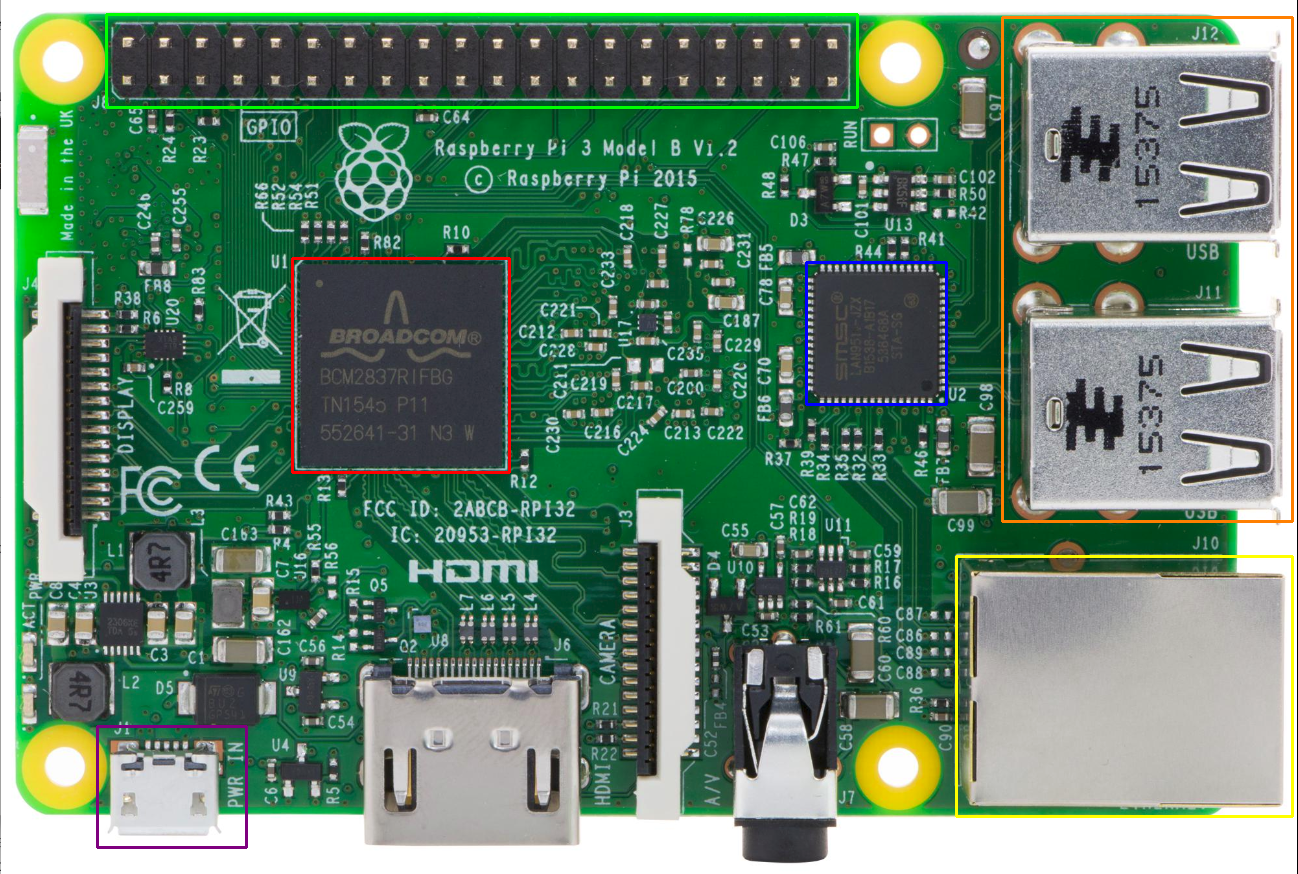
\includegraphics[width=\linewidth]{slike/rpi3_color.png}
  \caption{Raspberry Pi 3B.}
  \label{fig:rpi3}
\end{figure}

	\subsection{Sklopovlje}
		\paragraph{\underline{Glavni čipovi}} % (fold)
		\label{par:main_chips}
		
		Glavne procesne jedinice nalaze se u čipu Broadcom BCM2837, koji je na slici označen crvenim pravokutnikom. Riječ je o tzv. \textit{System-on-Chip} (SoC) čipu koji sadrži:
		\begin{itemize}
			\item \textbf{CPU} - 64-bitni ARMv8 Cortex A53 s četiri jezgre na 1.2 GHz,
			\item \textbf{GPU} - VideoCore IV na 400 MHz.
		\end{itemize}

		\par Taj je SoC spregnut s \textbf{radnom memorijom} s druge strane tiskane pločice. Riječ je o LPDDR2 SDRAM memoriji, s kapacitetom od 1 GB.

		\par Za bežičnu je komunikaciju zadužen procesor osnovnog pojasa (engl. \textit{baseband processor}) BCM43438, također od tvrtke Broadcom, koji podržava WiFi i Bluetooth 4.1 protokole. Smješten je na stražnjoj strani pločice, a spregnut je s antenom na prednjoj strani. Nije zgorega napomenuti da je Raspberry Pi 3 prva inačica ovog računala koja ima ugrađeno sklopovlje za bežičnu komunikaciju.

		\par Konačno, SMSC LAN9514 (na slici uokviren plavom bojom) vrši funkciju USB čvora i Ethernet upravljača. Povezan je s procesorom jednom USB vezom, pa sa svakim od četiri USB priključka, te s Ethernet priključkom procesor komunicira preko te USB veze.
		% paragraph glavni_cipovi (end)

		\paragraph{\underline{Ulazno-izlazni priključci}} % (fold)
		\label{par:IO_ports}
		
		Kao i svako drugo računalo, i RPi3 bi bio prilično beskoristan bez mogućnosti komunikacije s vanjskim svijetom. Naravno, na njemu postoji mnoštvo ulazno-izlaznih sučelja, a način na koji su ona izvedena je uvelike zaslužan za takvu popularnost ovog računala. Za ovaj seminar najvažniji priključci označeni su na Slici \ref{fig:rpi3}, a u nastavku je dan pregled tih sučelja:
		\begin{itemize}
			\item Četiri \textbf{USB 2.0} priključka [narančasti pravokutnik]
			\item Jedan \textbf{Ethernet} priključak [žuti pravokutnik]
			\item Jedan \textbf{microUSB} priključak - samo za napajanje, ne i za komunikaciju [ljubičasti pravokutnik]
			\item Četrdeset ulazno-izlaznih pinova opće namjene (\textbf{GPIO} - \textit{General Purpose Input/Output}) [zeleni pravokutnik]
			\item Ulaz za \textbf{\textit{microSD} karticu} (s druge strane pločice)
			\item Audio priključak i HDMI izlaz
			\item Poseban priključak za službenu Raspberry Pi kameru
			\item Poseban \textit{display} priključak
		\end{itemize}

		\par Od posebne su važnosti za ovaj rad GPIO pinovi. Oni, su, naime, ključni za komunikaciju sa senzorima koji će biti razmotreni kasnije u radu. Omogućuju najčešće korištene \textit{low-level} protokole za sklopovsku komunikaciju: \textbf{I$^2$C, TTL i SPI.} Naravno, sadrže i pinove za napajanje i uzemljenje sklopova, kao i pinove namijenjene za korisničku definiciju ponašanja.
		% paragraph ulazno_izlazni_priključci (end)

	\subsection{Programska podrška}
		Programska je podrška za RPi3, baš kao i sklopovlje, izvedena s ciljem jednostavnosti i fleksibilnosti korištenja. Budući da nije riječ o mikrokontroleru (poput, primjerice, popularnog Arduina), već o potpuno opremljenom računalu, očito je da RPi3 mora imati neki operacijski sustav (u nastavku: OS). On se u glavnini slučajeva nalazi na \textbf{\textit{microSD} kartici}, koja ima ulogu sekundarne memorije.\footnote{Moguće je pokrenuti OS i s, primjerice, nekog USB tvrdog diska, ali to nadilazi temu ovog seminara.} Ovdje kao najpopularniji OS za RPi u priču ulazi \textbf{Raspbian.} \\

		\par Raspbian je besplatan i otvoren operacijski sustav baziran na distribuciji Linuxa zvanoj "Debian". Ono zbog čega je Raspbian toliko popularan jest činjenica da je taj \textbf{OS optimiziran upravo za Raspberry Pi sklopovlje.}\footnote{Ovo se može zaključiti i iz imena distribucije, koje je \textit{portmanteau} pojmova "Raspberry Pi" i "Debian".} Drugim riječima, Raspbian je distribucija Linuxa koja:
		\begin{itemize}
			\item je vrlo jednostavna za instalaciju i dolazi potpuno opremljena za normalan računalni rad - uključujući i \textbf{grafičko korisničko sučelje} (\textit{GUI - Graphical User Interface}) 
			\item dolazi s već instaliranom programskom podrškom za komunikaciju sa specijaliziranim sklopovljem (poput GPIO pinova) - primjerice, \textbf{iz terminala, C-a ili Pythona.}
		\end{itemize}


	\subsection{Primjeri korištenja}
	Uzevši u obzir ranije spomenute prednosti RPi3 računala - cijena, pristupačnost i dimenzije - RPi računala najčešće nađu svoju primjenu u dva konteksta:
	\begin{itemize}
		\item u edukativnim projektima (pristupačnost i cijena)
		\item u ugradbenim sustavima (male dimenzije i cijena)
	\end{itemize}
	U nastavku su ukratko izložena dva primjera korištenja RPi3 računala. Primjeri su relativno jednostavni, ali dobro ilustriraju moguće koncepte korištenja tog računala.
	\\
	\paragraph{\underline{Pametna brava}} % (fold)
	\label{par:smart_lock}
		Pametne su brave koncept novijeg datuma, a označavaju autorizaciju ulaza osobe u neki prostor, i to ne koristeći (samo) klasični, mehanički ključ, nego korištenje kartica, lozinki, ili čak primjerice, prepoznavanja lica. Za implementaciju jedne takve brave može poslužiti bilo kakav mikrokontroler, i RPi3 bi svakako bio pretjeran za tako jednostavan zadatak, ali ono što bi moglo umanjiti taj \textit{overhead} jest, primjerice, praćenje pristupa prostoru pomoću logova, udaljeno upravljanje bravom, ili agregiranje više neovisnih zadataka slične složenosti na jednom RPi-ju.
		\par Računarska sekcija Kluba studenata elektrotehnike konkretno koristi Raspberry Pi 3 za agregiranje informacija o radu nekoliko servera, a u planu je spajanje NFC čitača (\textit{Near-Field Communication} - tehnologija beskontaktne komunikacije korištena u studentskim iskaznicama i bankovnim karticama) na taj isti RPi3, kako bi se na taj način autenticiralo osobe koje žele ući u sekciju.

	% paragraph smart_lock (end)

	\paragraph{\underline{Kućni VPN i WiFi pristupna točka}} % (fold)
	\label{par:home_vpn}
		U kontekstu komunikacijskih mreža, VPN (\textit{Virtual Private Network}) je protokol spajanja na mrežu koji omogućuje virtualno pristupanje mreži s drugog mjesta i prosljeđivanje svòg lokalnog prometa kroz taj "tunel" na način koji osigurava privatnost i sigurnost, kao i (do neke mjere) svojstva mreže (dozvole i zabrane, primjerice, ili simulacija lokalnog pristupa) kakva su na udaljenoj mreži na koju je korisnik VPN-om spojen. Implementacijski detalji VPN-a nipošto nisu trivijalni, i neće se dalje razmatrati u ovom radu, ali takav se sustav relativno bezbolno može upogoniti upravo koristeći Raspberry Pi, umjesto da se (samo?) za taj zadatak koristi neko (red veličine skuplje) računalo opće namjene.
		\par Još jedna zanimljiva mogućnost koju pruža RPi3 (ali ne i ranije inačice - barem ne bez dodatnog sklopovlja) jest postavljanje pristupne točke za WiFi, koja bi bežični promet prosljeđivala žičnoj Ethernet vezi. Tako se može, u nedostatku kompletnijeg i trajnijeg rješenja, ostvariti \textit{ad hoc} bežična mreža ili pojačivač signala.

	% paragraph home_vpn (end)

\newpage


\section{Senzori}
	Sada kada je definirano računalo koje će agregirati i analizirati očitanja senzora koje ćemo koristiti, vrijeme je da i o njima nešto rečemo. Slučaj koji promatramo jest \textbf{mjerenje vibracija} na mirnim površinama poput vrata, sa svrhom utvrđivanja \textbf{izvora} vibracija. Shodno tome, slijede kratki pregledi jednog akcelerometra - senzora za mjerenje relativnog ubrzanja - te jednog senzora glasnoće.
	Ipak, prije toga, radi lakšeg razumijevanja slijedi vrlo kratki opis dva ranije spomenuta \textit{low-level} komunikacijska protokola.

	\subsection{Komunikacijski protokoli}
	\paragraph{\underline{I$^2$C}} % (fold)
	\label{par:i2c}
		I$^2$C (engl. \textit{Inter-Integrated Circuit}) komunikacija je protokol za sinkronu serijsku komunikaciju. Odlikuje ga iznimna jednostavnost korištenja - za upogoniti I$^2$C komunikaciju potrebne su samo dva pina:
		\begin{itemize} 
			\item \textbf{SDA} (\textit{Serial DAta line}) - podatkovna linija
			\item \textbf{SCL} (\textit{Serial CLock}) - linija sa signalom takta, za sinkronizaciju.
		\end{itemize}
		Protokol omogućuje spajanje više uređaja s I$^2$C mogućnosti na istu sabirnicu, što znači da postoji i koncept adresiranja, kao i \textit{master-slave} arhitekture. Detalji implementacije toga su preširoki za ova rad, ali ukratko - svaki I$^2$C uređaj mora imati svoju, na sabirnici jedinstvenu adresu, koja se obično sastoji od dvije heksadekadske znamenke. 
		Ono što je jednostavnost uporabe žrtvovala jest mogućnost istovremene dvosmjerne (engl. \textit{full duplex}) komunikacije - budući da postoji samo jedna podatkovna linija, očito je da je to nemoguće, već je moguća samo \textbf{naizmjenična dvosmjerna (engl. \textit{half duplex})} komunikacija.
	% paragraph i2c (end)

	\paragraph{\underline{SPI}} % (fold)
	\label{par:spi}
		SPI (\textit{Serial Peripheral Interface}) je također protokol za sinkronu serijsku komunikaciju, ali nešto drugačije koncipiran (i, posljedično, implementiran) od I$^2$C-a. Također je zamišljen kao \textit{master-slave} arhitektura s jednim \textit{masterom}, a za komunikaciju koristi četiri pina:
		\begin{itemize}
			\item \textbf{SCLK} (\textit{Serial CLocK}) - linija sa signalom takta, za sinkronizaciju,
			\item \textbf{MOSI} (\textit{Master Output Slave Input}) - izlaz iz \textit{master} komponente i ulaz u \textit{slave} komponentu,
			\item \textbf{MOSI} (\textit{Master Output Slave Input}) - izlaz iz \textit{slave} komponente i ulaz u \textit{master} komponentu; također jedina linija koja ulazi u \textit{master} komponentu,
			\item \textbf{SS} (\textit{Slave Select}) - pin za adresiranje \textit{slave} komponente.
		\end{itemize}

		Budući da su u SPI protokolu prisutne dvije podatkovne linije, sada je već \textbf{moguća \textit{full duplex}} komunikacije, i to je ujedno glavna prednost SPI-a nad I$^2$C-om.
	% paragraph spi (end)

	\newpage
	\subsection{Akcelerometar - Adafruit LIS3DH}
		Tvrtka Adafruit se bavi razvojem otvorenog i pristupačnog sklopovlja, poglavito u edukativne svrhe. Tvrtka je od osnutka izdala na tržište mnoštvo vrlo raznolikih komponenti, a među njima i nekoliko akcelerometara. Jedan od njih je \textbf{LIS3DH}, vrlo popularan akcelerometar koji mjeri na 3 osi. Glavne karakteristike ovog sklopa su:
		\begin{itemize}
			\item mjerenje na \textbf{tri osi}
			\item \textbf{10-bitna} preciznost
			\item \textbf{I$^2$C i SPI} mogućnosti
			\item vrlo mala potrošnja
			\item vrlo niska cijena
		\end{itemize}

		\begin{figure}[h!]
			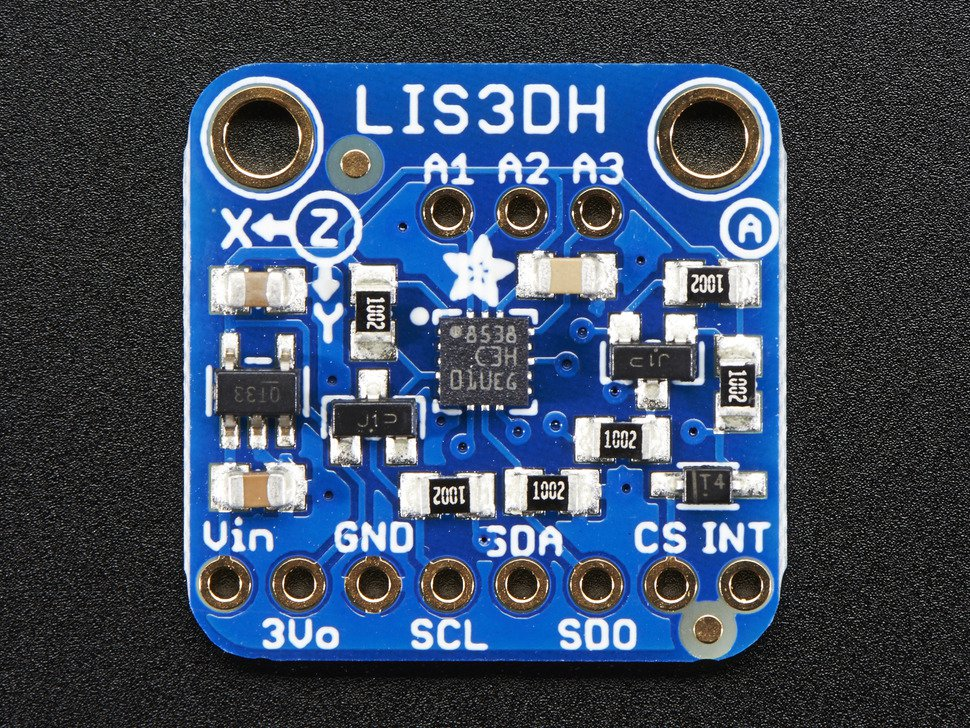
\includegraphics[width=\linewidth]{slike/lis3dh.jpg}
			\caption{Akcelerometar LIS3DH.}
			\label{fig:lis3dh}
		\end{figure}

		\par Ako se koristi I$^2$C, onda CS (\textit{Chip Select}) mora biti ili otpojen ili pritegnut na visoku naponsku razinu. U protivnom, ako se koristi SPI, onda CS mora biti pritegnut na masu.

		\par Sklop ima dvije moguće I$^2$C adrese - 0x18 i 0x19, tako da je moguće spojiti dva ovakva senzora na isti \textit{master}. Adresa se određuje tako da se pin SDO ostavi "u zraku" ili pritegne na nisku razinu za 0x18, odnosno na visoku razinu za 0x19. \\
		RPi3 u svojim GPIO pinovima ima dva para I$^2$C pinova - I$^2$C0 i I$^2$C1. Svejedno je koji se koristi, samo je ključno da se parovi ne pomiješaju - SDA0 mora biti uparen s SCL0, a ne s SCL1, recimo. Primjer I$^2$C spajanja prikazan je na Slici \ref{fig:lis3dhRpi} lijevo.

		\par Spajanje preko SPI-a izvodi se tako da je SCL i dalje u ulozi signala takta, ali je pin označen kao SDA sada u ulozi MOSI, a pin SDO u ulozi MISO pina. CS, kao što je već rečeno, za SPI mora biti uzemljen. Primjer SPI spajanja prikazan je na Slici \ref{fig:lis3dhRpi} desno.

		\begin{figure}[h!]
			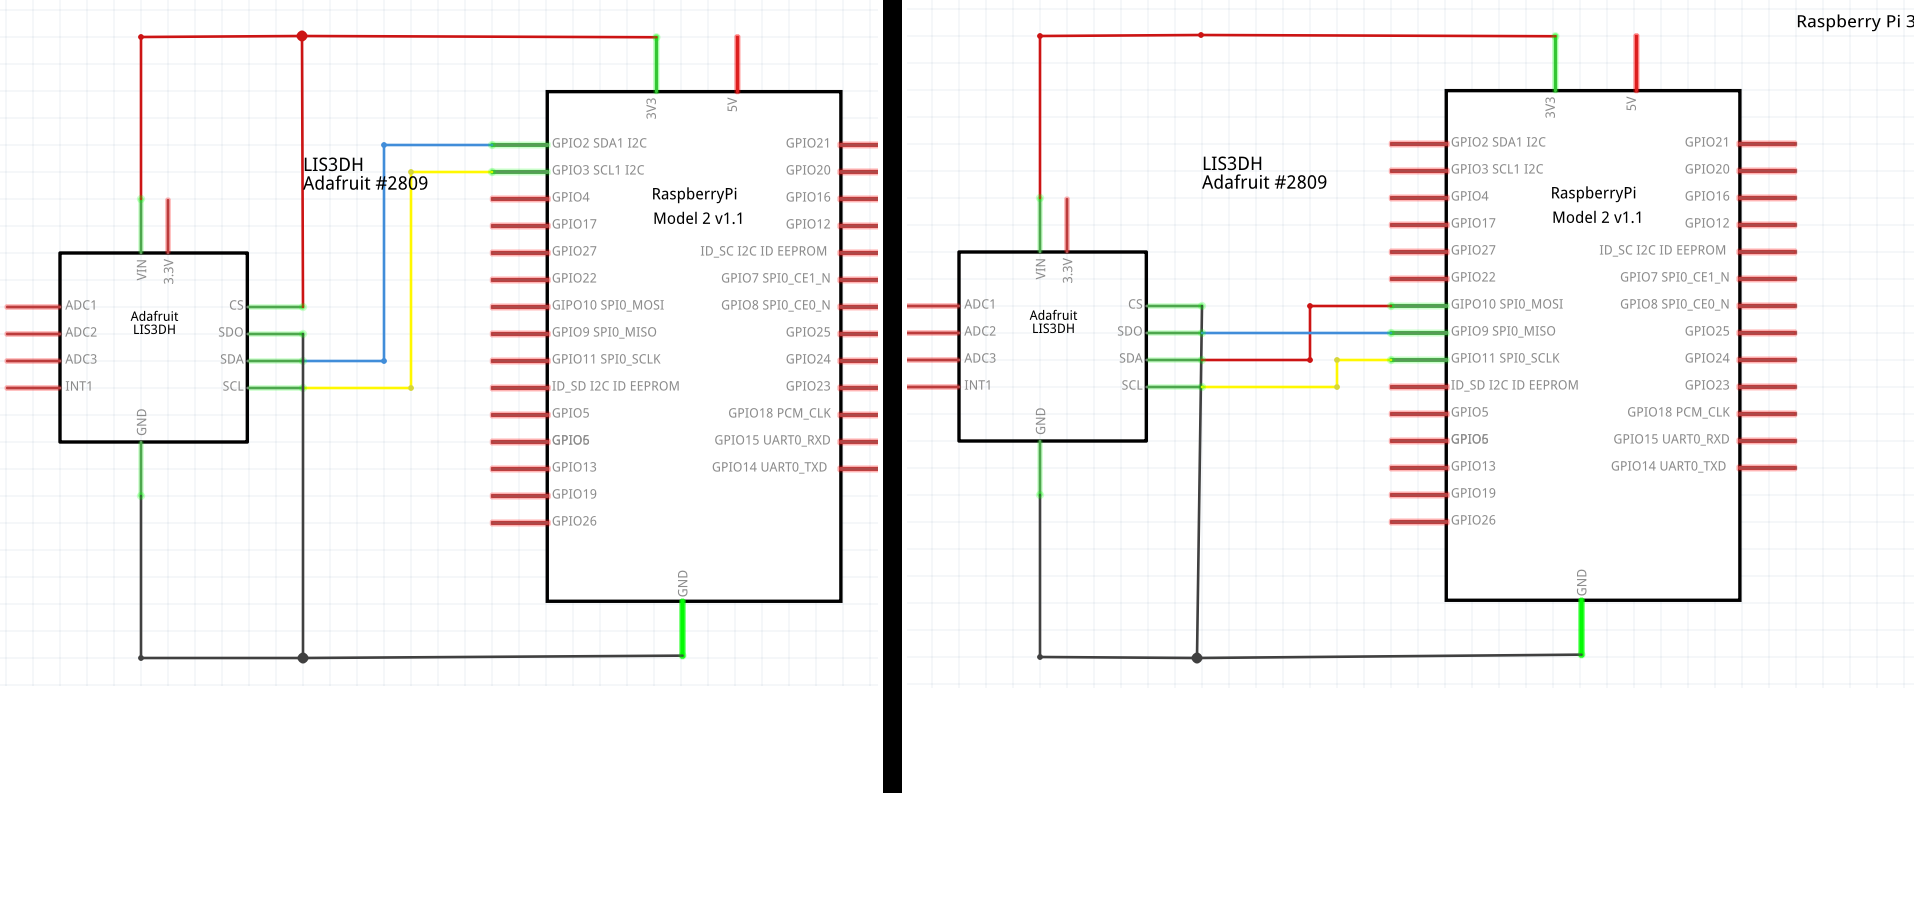
\includegraphics[width=\linewidth]{slike/i2cSpiMergeNoLabel.png}
			\caption{Primjer povezivanja LIS3DH i RPi3 - I$^2$C (lijevo) i SPI (desno).}
			\label{fig:lis3dhRpi}
		\end{figure}

		\par Ovime su ispunjeni sklopovski preduvjeti za osnovnu komunikaciju između senzora i RPi-ja, i za jednostavne primjere nije potrebno ništa više, ali ovaj senzor ima još nekoliko pinova koji nude interesantne mogućnosti:
		\begin{itemize}
			\item INT - \textbf{prekidni pin}
			\item A1, A2, A3 - analogno-digitalni pretvornici (engl. \textit{\textbf{ADC} - Analog-Digital Converter}) \\
		\end{itemize}

		Pinovi za ADC omogućuju da se na njih spoji neki analogni ulaz, koji će čip potom digitalizirati, s 10-bitnom preciznošću. Ovo se može pokazati pogodnim za situaciju u kojoj nemamo drugi ADC uređaj. 

		\par Prekidni pin omogućuje slanje prekidnog signala kao rezultat različitih događaja - senzor, naime, ima ugrađenu podršku za prepoznavanje jednostrukog i dvostrukog kuckanja, promjene orijentacije i slobodnog pada. Tu je podršku moguće iskoristiti kao okidač za generiranje prekida. Dakle, kada se dogodi neki događaj koji želimo pratiti (primjerice, kucanje po nekoj površini), sklop može generirati prekidni zahtjev da obavijesti RPi da je došlo do takvog događaja.

		\par \textbf{Primjer konfiguracije prekida?}


	\newpage
	\subsection{Mikrofon - Adafruit MAX4466?}
\newpage
\section{Pregled dostupnih programskih okvira}

\newpage
\section{Primjeri}
	\subsection{Programski kôd}
	\subsection{Očitani podaci}

\newpage
\section{Zaključak}

\newpage
\section{Literatura}

\begin{itemize}
	\item Raspberry Pi službene stranice: \url{https://www.raspberrypi.org/}
	\item ADXL345: \url{https://learn.adafruit.com/adxl345-digital-accelerometer}
	\item MMA8451: \url{https://learn.adafruit.com/adafruit-mma8451-accelerometer-breakout/wiring-and-test?view=all}
	\item LIS3DH: \url{https://learn.adafruit.com/adafruit-lis3dh-triple-axis-accelerometer-breakout/downloads?view=all}
	\item Zvučni senzori: \url{https://www.sunfounder.com/learn/sensor-kit-v2-0-for-raspberry-pi-b-plus/lesson-19-sound-sensor-sensor-kit-v2-0-for-b-plus.html}
\end{itemize}

\end{document}
